\documentclass[12pt,a4paper]{article}
\usepackage{amssymb, amsmath}
\usepackage{theorem}
\usepackage{clrscode}
\usepackage{fullpage}
\usepackage{graphicx}
\usepackage{enumitem}

\setlength{\parskip}{0cm}
\setlength{\parindent}{0pt}
\newtheorem{thm}{Theorem}

\pagestyle{empty}

\begin{document}

\begin{center}
  
  \bigskip \bigskip

  {\huge \textbf{Machine Learning}}

  \bigskip
  
  {\large Spring 2020}

  \bigskip \bigskip

  {\large \textsc{Homework 1}} 
  
  \bigskip \bigskip
  
  {\large \textbf{Ozren Dabić}}
  
  \bigskip \bigskip
  
  {\small \textbf{In collaboration with: Marco Paganoni and Pasquale Polverino}}
  
  \bigskip \bigskip

\end{center}

\section*{Tasks}
\subsection*{T1}

Please refer to \textit{t1.py} to see how I implemented the solution in python. To summarise the implementation, \textit{t1.py} does the following:
\begin{enumerate}
\itemsep-0.25em 
	\item It first loads the $X$ and $y$ value dataset from \textit{data.nz}, using the data loader function provided in \textit{run\_model.py};
	\item It then splits the $X$ and $y$ data into the training and test sets, using the \textit{train\_test\_split} function, imported from \textit{sklearn}. I split the sets according to how it was presented in the lecture slides. Given that our dataset has roughly 1200 data points, the test data set would be comprised of $15\%$ of that data. The ``random state'' is just to ensure that one seed is constantly used, so that the results are consistent;
	\item Then, the family of models, specified in the task description is defined. To achieve this an \textit{sklearn.pipeline} is constructed. The pipeline is used to add the regressor, using the \textit{FunctionTransformer}, coupled with the appropriate transformation function\footnote{I had to define the transformation function in \textit{run\_model.py}, as the pickle file could not be unpacked if the function was not present in said file. The \textit{transform} function simply appends $\sin(x_1) * x_2$ to each data point.} passed to its constructor.
	\item We then fit the model, using \textit{LinearRegression}'s \textit{fit} function, and save the model to \textit{t1.pickle} in the \textit{deliverable} directory.
\end{enumerate}

The estimates for the model parameters I obtained were:\\
$\hat{\theta_0} =  1.5457$\\
$\hat{\theta_1} = -0.1996$\\
$\hat{\theta_2} = -0.3625$\\
$\hat{\theta_3} = -0.1273$\\

Which yield the following model formula:

\begin{equation*}
f(x,\hat{\theta}) = 1.5457 - 0.1996 \cdot x_1 - 0.3625 \cdot x_2 - 0.1273 \cdot (sin(x_1) \cdot x_2)
\end{equation*}

And by evaluating the predictions made on the given samples, the performance is \\$MSE = 0.2068$.

\newpage
\subsection*{T2}

Please refer to \textit{t2.py} to see how I implemented the solution in python. The implementation follows a similar pattern to that displayed in \textit{t1.py}, namely how the data is loaded, partitioned, and how the model is stored once fit. The only difference lies in the regression model used. Since the task requires a non-linear regression model, the \textit{sklearn} \textit{LinearRegression} model is substituted with a feedforward neural network, implemented using \textit{KerasRegressor} from \textit{keras}. The neural network implementation draws heavy inspiration from the example on our course repository, using two layers with nonlinear activation function, and a single, linear output layer.
\\\\
By evaluating the predictions made on the given samples, the performance is\\$MSE \approx 0.015$.\\\\
Comparing the obtained performance measure to the one from \textbf{T2}, it's easy to see that the feedforward neural network performs much better (nearly 10 times better in fact). This is not all that surprising, given that linear models don't fit non-linear data as accurately as non-linear models do.

\newpage
\section*{Questions}

\subsection*{Training versus Validation}

\begin{figure}[h!]
\begin{center}    
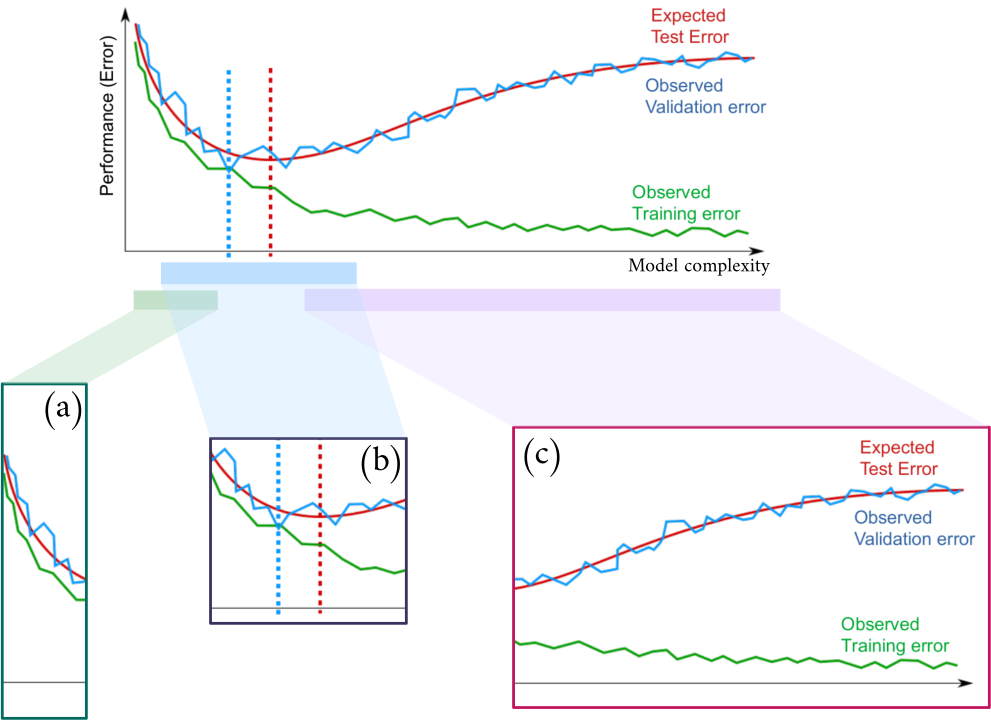
\includegraphics[width=1\textwidth,keepaspectratio]{figures/figure1}
\end{center}
\caption{This is what you missed last class}
\end{figure}

\subsubsection*{What is the whole figure about?}

This figure represents the relationship between the approximation performance and model complexity of a linear regression model.

\subsubsection*{Explain the curves' behaviour in each of the three highlighted sections of the figures!}

First let's explain what each of the curves represents. When training our linear regression model, we spit our data into 3 sets: the training, validation and test set. The training set is used exclusively to train the model, while the test set is used to determine accuracy of said training. The validation set is used to determine how well the model generalises unseen data. Observing the graph, we notice that the error of all 3 performance measures is high when model complexity is low. The model simply has not trained enough to make accurate predictions for either seen or unseen data. 
\newpage
As model complexity increases, so does the accuracy of the model. Two vertical lines are observable in this section. They represent the optimal models, according to the validation and test set respectively. As model complexity increases further, the training set performance increases, but the validation and test set performance decrease. This is because the model is overtrained to generalise data according to the training set, preventing it from making correct generalisations when being fed the (unseen) validation data.

\subsubsection*{Is any of the three section associated with the concepts of overfitting and underfitting?}

\begin{enumerate}[label=\alph*)]
\itemsep-0.25em 
	\item This section illustrates the consequence of a model suffering from underfitting. Due to a lack of training, underfit models can not accurately model the training data. As a result, regression never picks up the trend present in the data, leading to unreliable predictions.
	\item An optimal model, is a model that generalises well. Such a model is neither underfit nor overfit. This section represents an optimal model of our validation set and test set, both lines pointing to the exact model complexity required for the two sets to be considered optimal.
	\item While section a) was dedicated to underfitting, this final section displays the case of overfitting. While a lack of training can negatively effect predictions, too much training can also have a negative impact. Overfitting occurs in such a case, when a model learns the training data too well, leading to unreliable generalisations (hence the huge performance disparity between the observed training error and the validation/test error). The purpose of regression is to capture and fit the data according to a dominant trend, not according to all trends.
\end{enumerate}

\subsubsection*{What is early stopping?}

Early stopping is a method for controlling model complexity, with the central goal of avoiding overfitting. Early stopping rules provide guidance as to how many iterations can be run before the learner begins to over-fit. To find this ideal number of iterations, one must observe when the training set error begins to deviate from the validation set error, as the deviation is a clear sign of a model entering the overfitting stage.

\newpage
\subsection*{Logistic Regression}

\subsubsection*{1)}

The logistic activation function\footnote{Whereas: $l(x,\theta) = \theta_0 + \theta_1 \cdot x_1 \cdot x_2 + \theta_2 \cdot \sin(x_1)$} of a neutron is expressed as:

\begin{equation*}
	\text{logistic}(l(x,\theta)) = \frac{1}{1+e^{-l(x,\theta)}}
\end{equation*}

Therefore, the binary cross-entropy loss equates to:

\begin{equation*}
	V_n(\theta) = - \frac{1}{n} \displaystyle \sum_{i=1}^n \lbrack y_i \cdot \text{logistic}(l(x_i,\theta)) + (1 - y_i) \cdot (1 - \text{logistic}(l(x_i,\theta))) \rbrack
\end{equation*}

With $V_n$ defined, we can also define its gradient w.r.t. $\theta$:

\begin{equation*}
	\triangledown_\theta V_n(\theta) = 
	\begin{bmatrix}
		\frac{\partial V_n (\theta)}{\partial \theta_0} & \frac{\partial V_n (\theta)}{\partial \theta_1} & \frac{\partial V_n (\theta)}{\partial \theta_2} \\
	\end{bmatrix}^{T}
\end{equation*}

By computing the partial derivatives, we get:

\begin{equation*}
\triangledown_\theta V_n(\theta) 
=
-\frac{1}{n}
\begin{bmatrix}
    \sum_{i=1}^n [ \frac{y_i e^{-l(x_i,\theta)}}{1+e^{-l(x_i,\theta)}} - \frac{(1-y_i)}{1+e^{-l(x_i,\theta)}} ] \\\\
    \sum_{i=1}^n [ \frac{y_i x_1 x_ 2 e^{-l(x_i,\theta)}}{1+e^{-l(x_i,\theta)}} - \frac{x_1x_2(1-y_i)}{1+e^{-l(x_i,\theta)}} ] \\\\
    \sum_{i=1}^n [ \frac{y_i \sin(x_1) e^{-l(x_i,\theta)}}{1+e^{-l(x_i,\theta)}} - \frac{\sin(x_1)(1-y_i)}{1+e^{-l(x_i,\theta)}} ] \\
\end{bmatrix}
\end{equation*}

Which is further simplified to:

\begin{equation*}
\triangledown_\theta V_n(\theta) 
=
-\frac{1}{n}
\displaystyle \sum_{i=1}^n
\begin{bmatrix}
	y_i - \text{logistic}(l(x_i,\theta))
\end{bmatrix}
\begin{bmatrix}
    1\\
    x_1x_2\\
    \sin(x_1)\\
\end{bmatrix}
\end{equation*}

\begin{equation*}
\triangledown_\theta V_n(\theta) 
=
-\frac{1}{n}
\displaystyle \sum_{i=1}^n
\begin{bmatrix}
	y_i - \text{logistic}(l(x_i,\theta))
\end{bmatrix}
\triangledown_\theta l(x,\theta)
\end{equation*}

\subsubsection*{2)}

The main difference between a perceptron and a logistic-function neuron lies in which activation functions they use. While a perceptron uses the Heaviside step function, defined as:
\begin{equation*}
H(x) = 
\begin{cases}
    0 & \text{if $x < 0$}\\
    1 & \text{otherwise}
\end{cases}
\end{equation*}

The logistic-function neuron uses the sigmoid function, defined as:
\begin{equation*}
\sigma(x) = \dfrac{1}{1+e^{-x}}
\end{equation*}

\newpage
The major limit that the perceptron and the logistic-function neuron share is that they are unable to solve non-linearly separable problems. Neural networks circumvent this problem by stacking multiple perceptron or logistic-function neuron layers.
\\\\
The purpouse of activation functions, is to serve as mathematical “gate” in between the input feeding the current neuron, and its output going to the next layer. Each layer applies separate weights to the input, as well as a bias measurement.

\subsection*{Processing}

The goal of normalisation is to change the values of numeric columns in the dataset to a common scale, without distorting differences in the ranges of values. This is why normalising features appears to be preferable, as balancing features to have similar ranges to each other, allows us to make better estimates. Since Lasso and Ridge place constraints on the size of the coefficients associated to each variable, it is not only preferable, but necessary to normalise, as the value of the coefficients will depend on the magnitude of each variable.

\end{document}
